}\label{logbook}

\begin{longtable}[]{@{}
  >{\raggedright\arraybackslash}p{(\columnwidth - 0\tabcolsep) * \real{1.0000}}@{}}
\toprule\noalign{}
\begin{minipage}[b]{\linewidth}\raggedright
\textbf{Weekly/} \textbf{Fortnightly Log Entry}

\textbf{Project Title: Machine Learning Models using the Mixed Signals
Dataset}

\textbf{Supervisor: Mao Shan}

\textbf{Date: 08/03/2026}

\textbf{Meeting Time: 3:30 PM 2/3/2026, 29/1/2026}

Do thesis work on an applied industry problem that could only be done by
me with this one data set and with this supervisor only to get most
value.

\url{https://mixedsignalsdataset.cs.cornell.edu/download/}

MS3D++ refers to a multi sensor 3D detection and self training
framework, designed to improve 3d object performance,~

MS3D type study: \url{https://github.com/darrenjkt/MS3D}

\begin{enumerate}
\def\labelenumi{\arabic{enumi}.}
\item
  Baseline detector
\end{enumerate}

CO3 - \url{https://github.com/Runjian-Chen/CO3}

\begin{enumerate}
\def\labelenumi{\arabic{enumi}.}
\item
  \textbf{Objectives}
\end{enumerate}

\begin{itemize}
\item
  Discussed Mixed Signals and Possible paths to go down with Mixed
  Signals
\item
  Cooperative Perception, Predictive Perception,
\end{itemize}

\begin{enumerate}
\def\labelenumi{\arabic{enumi}.}
\setcounter{enumi}{1}
\item
  \textbf{Activities Performed}
\end{enumerate}

Research about 3D object detectors. Point Cloud and Lidar. Orin Nano AI
supercomputer

\begin{enumerate}
\def\labelenumi{\arabic{enumi}.}
\setcounter{enumi}{2}
\item
  \textbf{Data / Results / Plots / Diagrams / Equations}
\end{enumerate}

n/a

\begin{enumerate}
\def\labelenumi{\arabic{enumi}.}
\setcounter{enumi}{3}
\item
  \textbf{Observations and Reflections}
\end{enumerate}

n/a

\begin{enumerate}
\def\labelenumi{\arabic{enumi}.}
\setcounter{enumi}{4}
\item
  \textbf{Problems Encountered}
\end{enumerate}

n/a

\begin{enumerate}
\def\labelenumi{\arabic{enumi}.}
\setcounter{enumi}{5}
\item
  \textbf{Next Steps / To-Do List (max 50 words)}
\end{enumerate}

Research about 3D object detectors. Point Cloud and Lidar.

\begin{enumerate}
\def\labelenumi{\arabic{enumi}.}
\setcounter{enumi}{6}
\item
  \textbf{Appendices / Reference Notes (optional)}
\end{enumerate}
\end{minipage} \\
\midrule\noalign{}
\endhead
\bottomrule\noalign{}
\endlastfoot
\begin{minipage}[t]{\linewidth}\raggedright
\textbf{Weekly/} \textbf{Fortnightly Log Entry}

\textbf{Project Title: Machine Learning Models using the Mixed Signals
Dataset to For Static Mapping remove Occlusion}

\textbf{Supervisor: Mao Shan}

\textbf{Date: 20/03/2026}

\textbf{Meeting Time: 3:30 PM 20/3/2026}

Had a meeting with Steffany Berrioz and Mao Shan. I have completed the
data set visualization. We discussed that 3D image detection may not be
suitable for a thesis. There may be potential in mapping of the static
environment, and occlusion of objects. We discussed the importance of
matrix fusion, high fidelity and clean map. Coordinate system fusion.
Coordinate Frame Fusion.

\textbf{Topic: Multi-LiDAR Autonomous Exploration and Mapping for
Occlusion Removal from Point Cloud}

\begin{enumerate}
\def\labelenumi{\arabic{enumi}.}
\item
  \textbf{Objectives}
\end{enumerate}

To create a draft of the proposal by Wednesday, Submit it on Friday.

Read papers on matrix fusion.

\begin{enumerate}
\def\labelenumi{\arabic{enumi}.}
\setcounter{enumi}{1}
\item
  \textbf{Activities Performed}
\end{enumerate}

Research about 3D object detectors. Point Cloud and Lidar. Preliminary
work on partial occlusion.

Mixed Signals Devkit.

\begin{enumerate}
\def\labelenumi{\arabic{enumi}.}
\setcounter{enumi}{2}
\item
  \textbf{Data / Results / Plots / Diagrams / Equations}
\end{enumerate}

n/a

\begin{enumerate}
\def\labelenumi{\arabic{enumi}.}
\setcounter{enumi}{3}
\item
  \textbf{Observations and Reflections}
\end{enumerate}

n/a

\begin{enumerate}
\def\labelenumi{\arabic{enumi}.}
\setcounter{enumi}{4}
\item
  \textbf{Problems Encountered}
\end{enumerate}

n/a

\begin{enumerate}
\def\labelenumi{\arabic{enumi}.}
\setcounter{enumi}{5}
\item
  \textbf{Next Steps / To-Do List (max 50 words)}
\end{enumerate}

n/a

\begin{enumerate}
\def\labelenumi{\arabic{enumi}.}
\setcounter{enumi}{6}
\item
  \textbf{Appendices / Reference Notes (optional)}
\end{enumerate}

n/a
\end{minipage} \\
\begin{minipage}[t]{\linewidth}\raggedright
\textbf{Weekly/} \textbf{Fortnightly Log Entry}

\textbf{Project Title: Machine Learning Models using the Mixed Signals
Dataset}

\textbf{Supervisor: Mao Shan}

\textbf{Date: 27/03/2026}

\textbf{Meeting Time: 10:30 AM 27/3/2026 -- Week 5}

\begin{enumerate}
\def\labelenumi{\arabic{enumi}.}
\item
  \textbf{Objectives}
\end{enumerate}

n/a

\begin{enumerate}
\def\labelenumi{\arabic{enumi}.}
\setcounter{enumi}{1}
\item
  \textbf{Activities Performed}
\end{enumerate}

n/a

\begin{enumerate}
\def\labelenumi{\arabic{enumi}.}
\setcounter{enumi}{2}
\item
  \textbf{Data / Results / Plots / Diagrams / Equations}
\end{enumerate}

n/a

\begin{enumerate}
\def\labelenumi{\arabic{enumi}.}
\setcounter{enumi}{3}
\item
  \textbf{Observations and Reflections}
\end{enumerate}

n/a

\begin{enumerate}
\def\labelenumi{\arabic{enumi}.}
\setcounter{enumi}{4}
\item
  \textbf{Problems Encountered}
\end{enumerate}

n/a

\begin{enumerate}
\def\labelenumi{\arabic{enumi}.}
\setcounter{enumi}{5}
\item
  \textbf{Next Steps / To-Do List (max 50 words)}
\end{enumerate}

n/a

\begin{enumerate}
\def\labelenumi{\arabic{enumi}.}
\setcounter{enumi}{6}
\item
  \textbf{Appendices / Reference Notes (optional)}
\end{enumerate}

n/a
\end{minipage} \\
\begin{minipage}[t]{\linewidth}\raggedright
\textbf{Weekly/} \textbf{Fortnightly Log Entry}

\textbf{Project Title: Occlusion Labelling for V2X}

\textbf{Supervisor: Mao Shan}

\textbf{Date: 11/04/2026}

\textbf{Meeting Time: 10:30 AM 3/4/2026, 10:30 AM 10/4/2026}

\begin{enumerate}
\def\labelenumi{\arabic{enumi}.}
\item
  \textbf{Objective}
\end{enumerate}

Goals that were completed were getting point cloud data and visibility
rating from an ego vehicle's perspective. Reflecting on the meeting, in
the first meeting I gained feedback on the proposal and what things I
could change. Mao gave me some feedback about what I could change and
what direction I can go down with occlusions. In the last meeting, I
went over my results that I found from the data and discussed some off
the shelf 3D detectors I could use to measure the effectiveness of the
metrics.

Some keypoints brought up were, objectives and aims of the research,
identify reliable metrics to quantify the occlusion in the points
clouds, quantitively analyse the occlusion based on performance from
object detectors.

\begin{enumerate}
\def\labelenumi{\arabic{enumi}.}
\setcounter{enumi}{1}
\item
  \textbf{Activities Performed}
\end{enumerate}

n/a

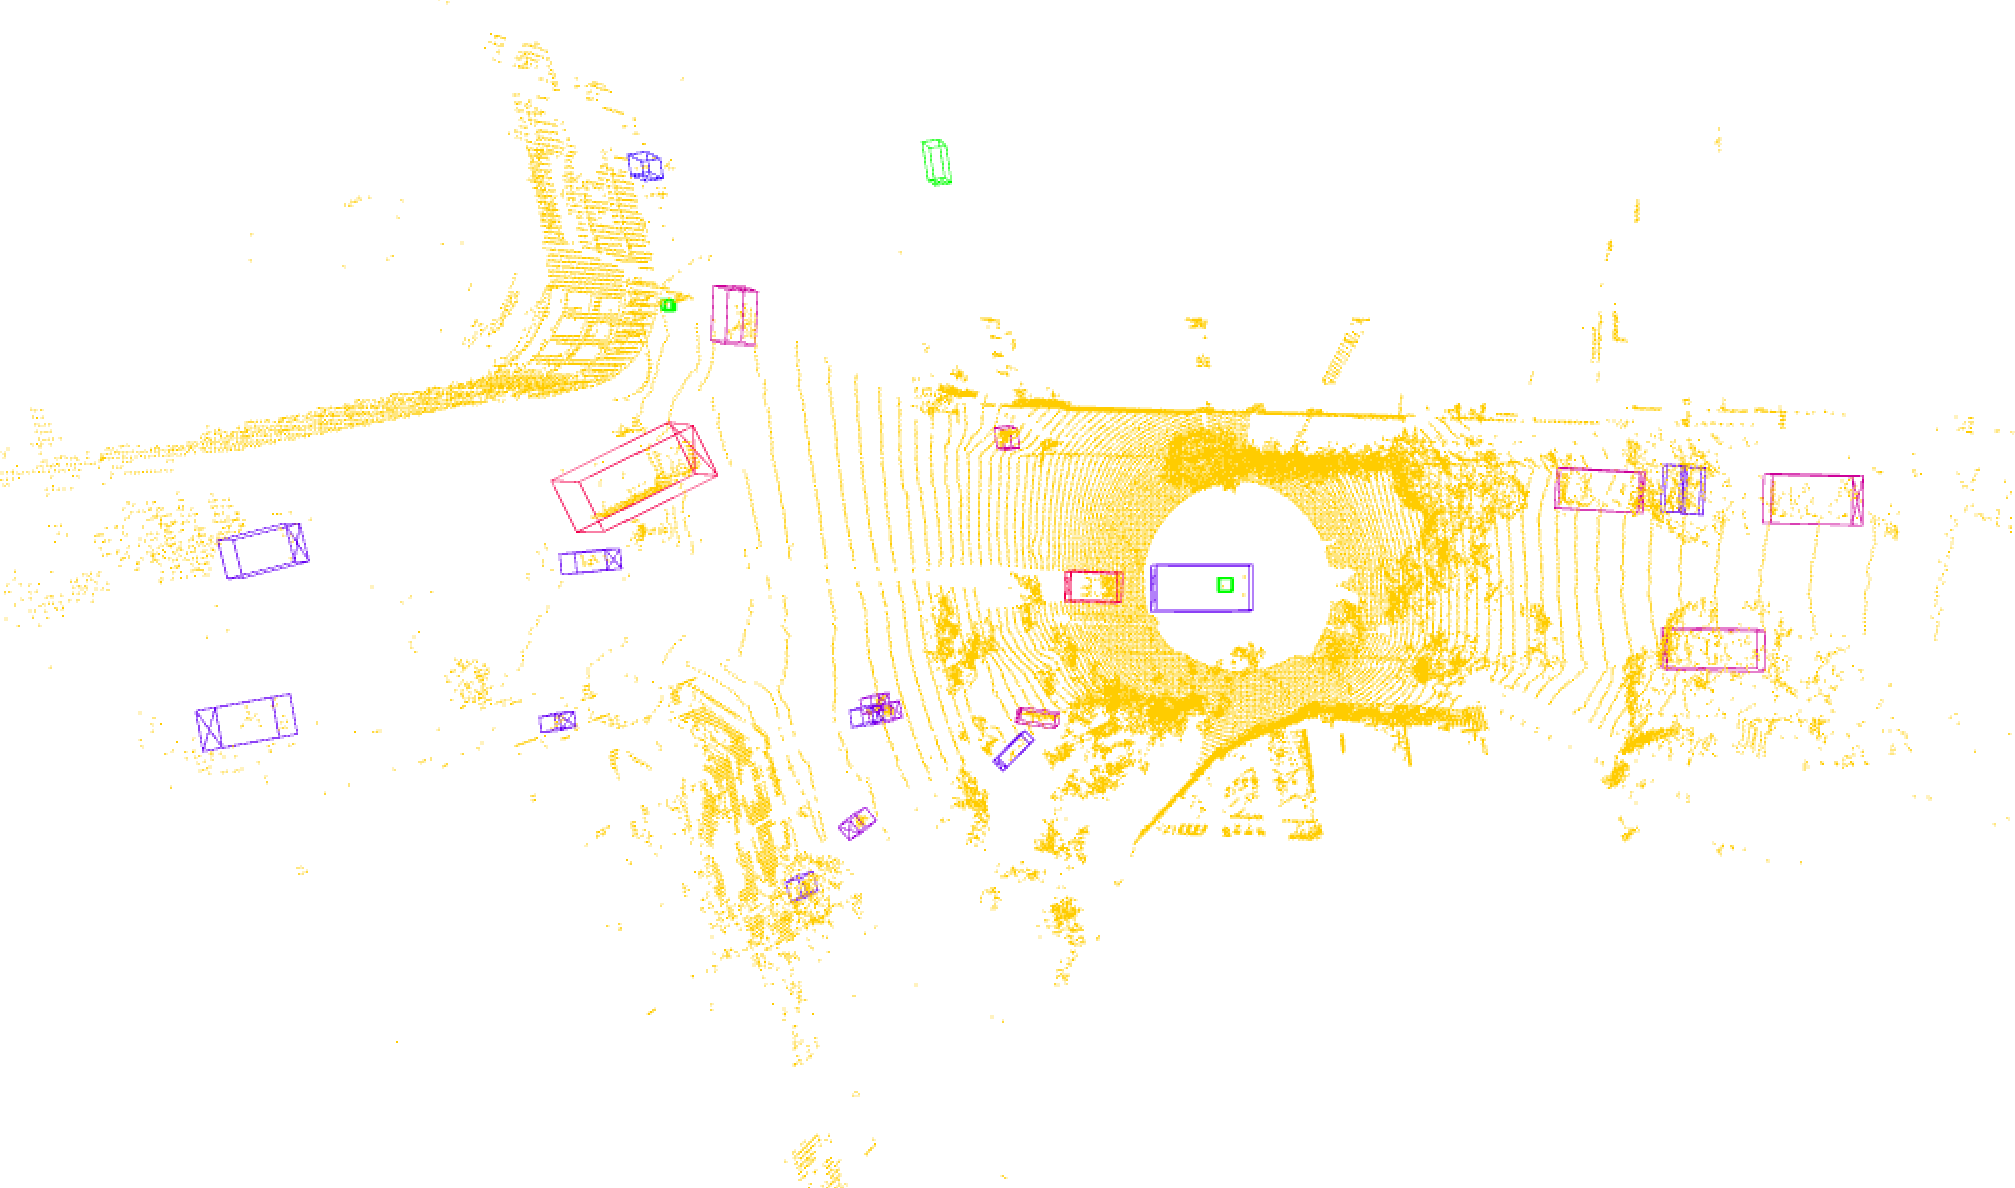
\includegraphics[width=3.70515in,height=2.18429in]{figures/image11.png}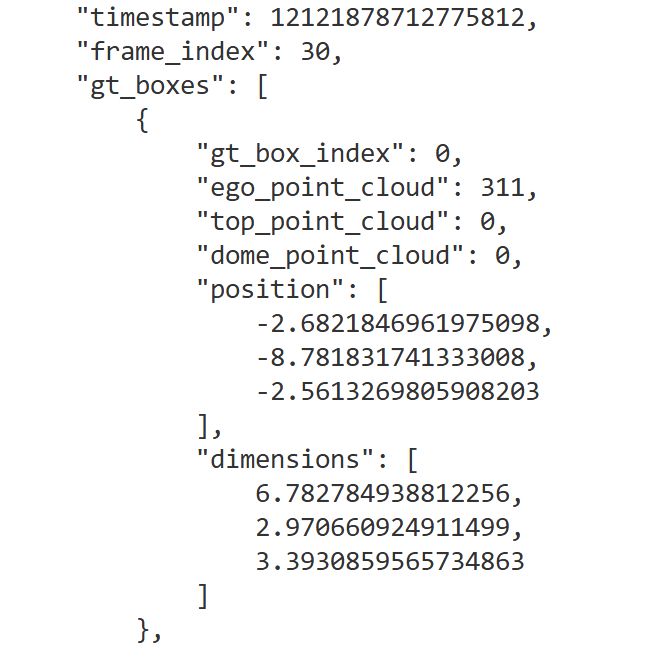
\includegraphics[width=2.25472in,height=2.23063in]{figures/image12.png}

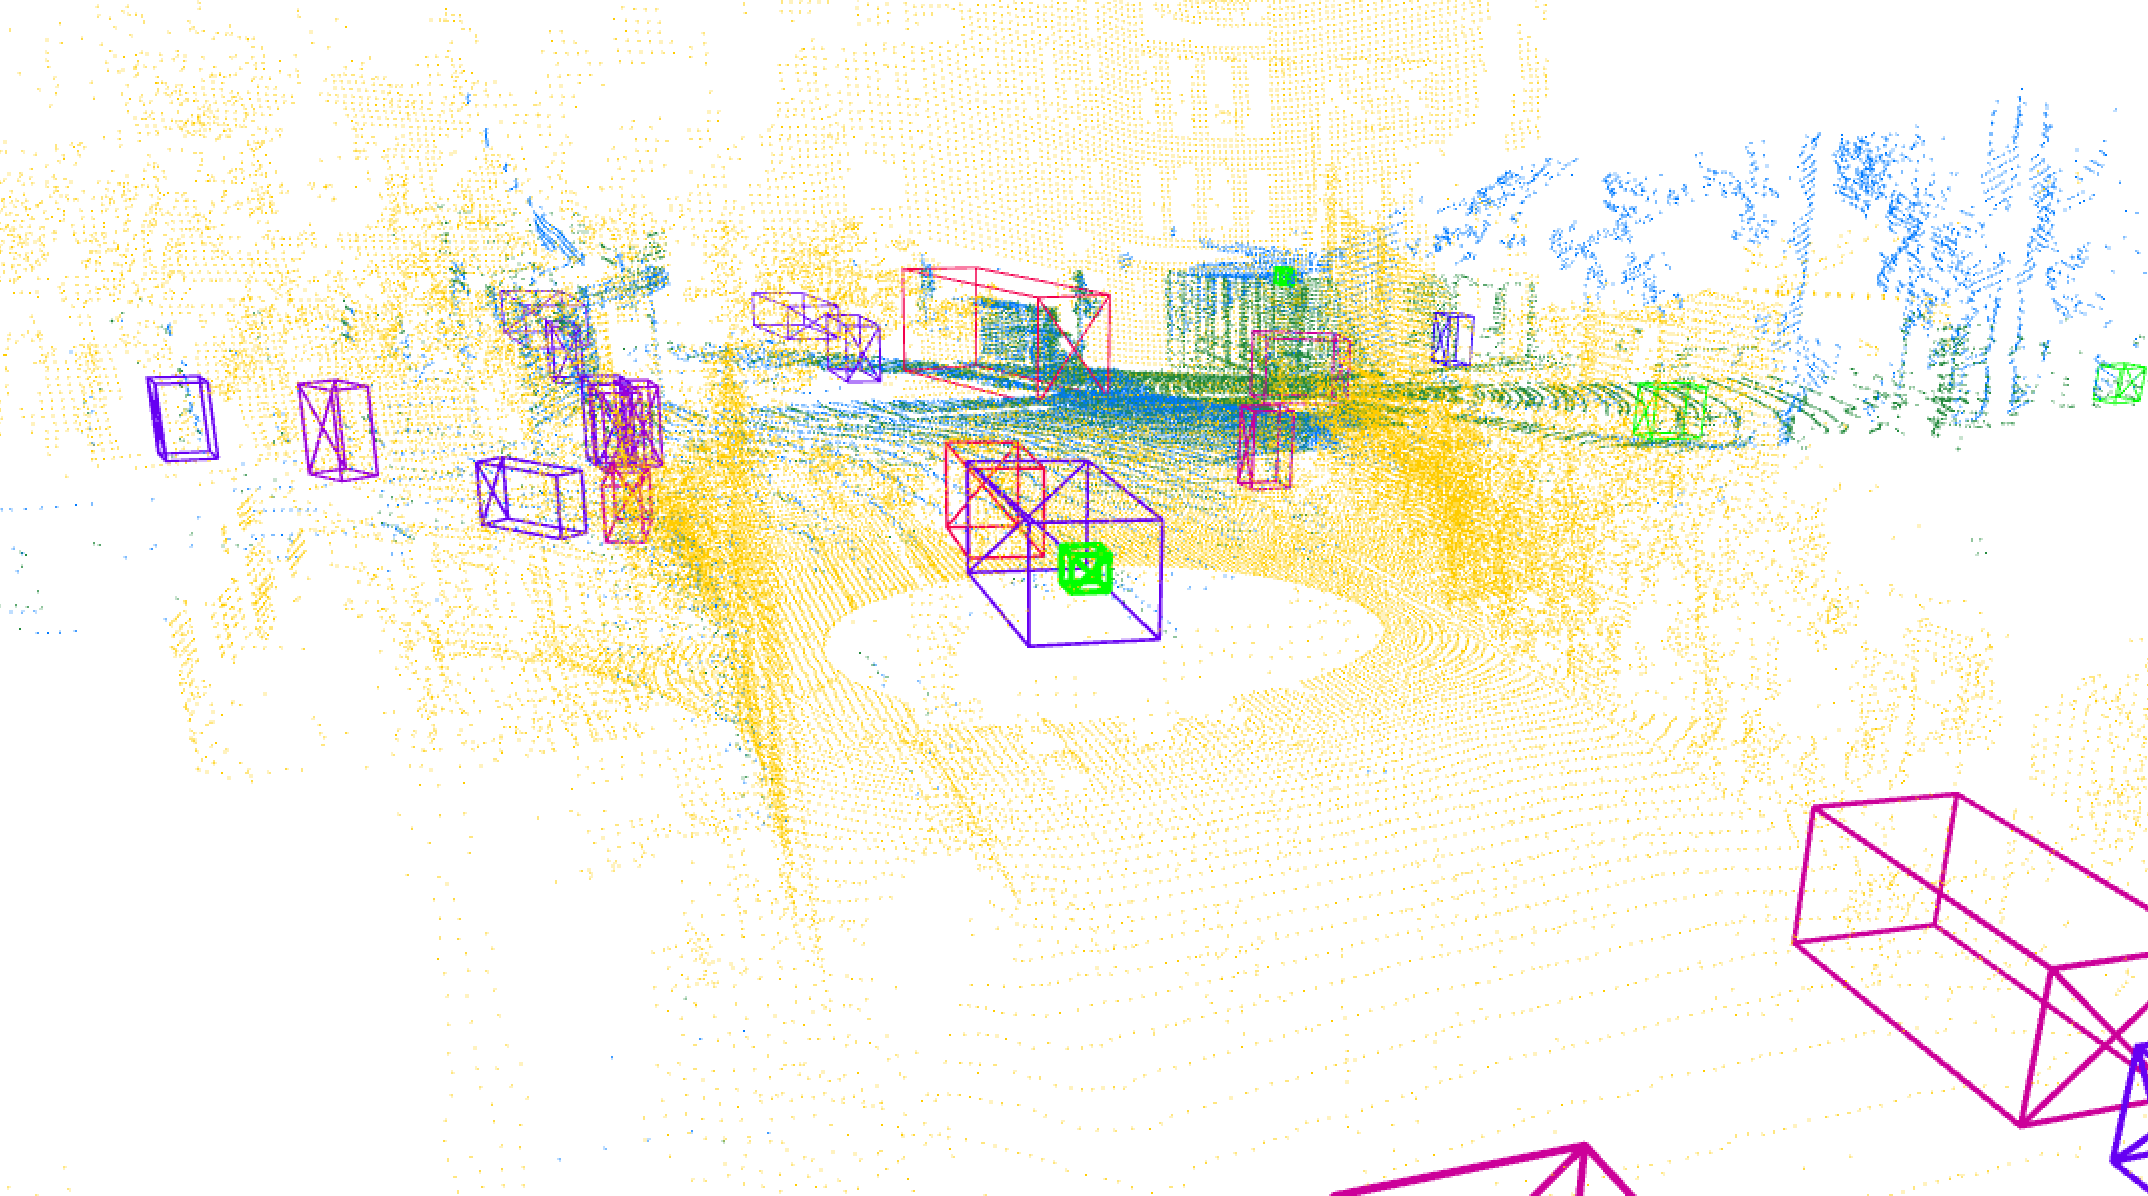
\includegraphics[width=3.32261in,height=1.85015in]{figures/image13.png}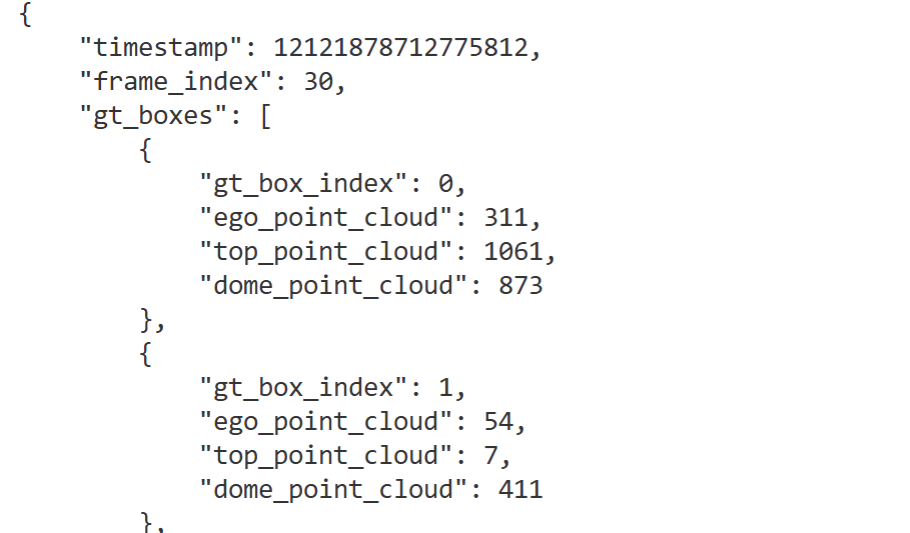
\includegraphics[width=2.22423in,height=1.30293in]{figures/image14.png}

Gathered some basic metrics from the data where I found the number of
intersecting point clouds and ground truth boxes. This gave me some
insights into developing some metrics that I can come up with to
quantify the occlusion.

\begin{enumerate}
\def\labelenumi{\arabic{enumi}.}
\setcounter{enumi}{2}
\item
  \textbf{Data / Results / Plots / Diagrams / Equations}
\end{enumerate}

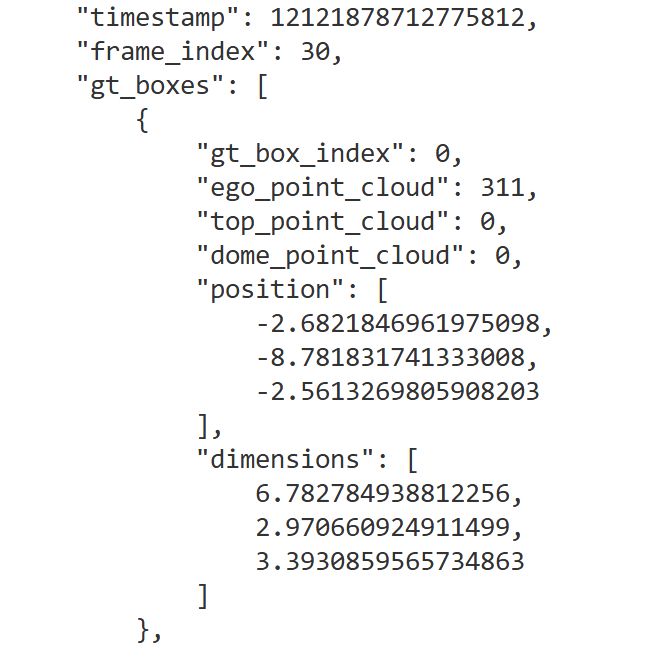
\includegraphics[width=2.25472in,height=2.23063in]{figures/image12.png}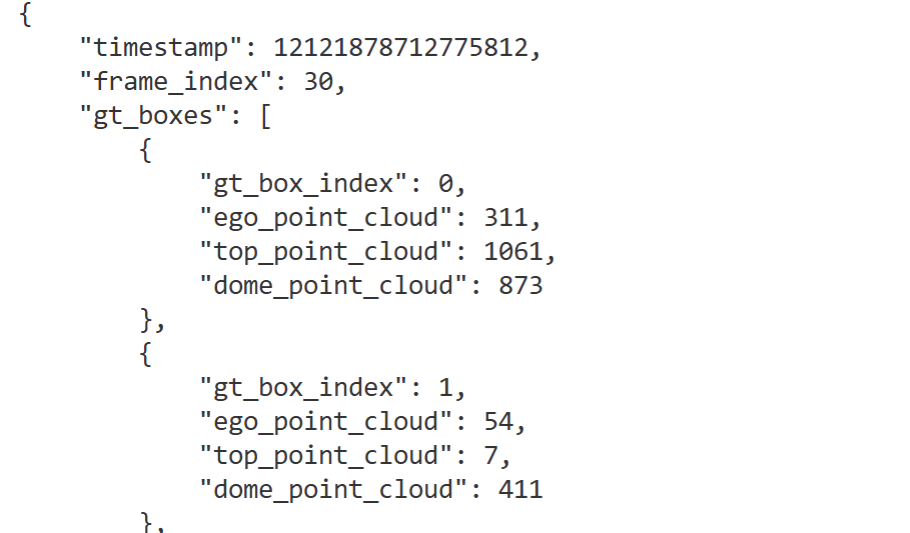
\includegraphics[width=3.37201in,height=1.97529in]{figures/image14.png}

\begin{enumerate}
\def\labelenumi{\arabic{enumi}.}
\setcounter{enumi}{3}
\item
  \textbf{Observations and Reflections}
\end{enumerate}

Some insights that I gained were that it is a good idea to revise the
proposal and come back to it as a reference and change as I go.

\begin{enumerate}
\def\labelenumi{\arabic{enumi}.}
\setcounter{enumi}{4}
\item
  \textbf{Problems Encountered}
\end{enumerate}

n/a

\begin{enumerate}
\def\labelenumi{\arabic{enumi}.}
\setcounter{enumi}{5}
\item
  \textbf{Next Steps / To-Do List (max 50 words)}
\item
\end{enumerate}

Next steps would be to put together a literature review. Also use
endnote to make my source accurate. Use Mendeley.

\begin{enumerate}
\def\labelenumi{\arabic{enumi}.}
\setcounter{enumi}{7}
\item
  \textbf{Appendices / Reference Notes (optional)}
\end{enumerate}

n/a
\end{minipage} \\
\begin{minipage}[t]{\linewidth}\raggedright
\textbf{Weekly/} \textbf{Fortnightly Log Entry}

\textbf{Project Title:} LiDAR Based Occlusion Metric for Autonomous
Vehicles in Urban Environments

\textbf{Supervisor: Mao Shan}

\textbf{Date: 24/04/2026}

\textbf{Meeting Time/s: 10:30-11 AM 24/4/2026}

\textbf{Meeting Minutes:}

\emph{Preliminary Report:}

Ordering: lidar, datasets, 3d object detection, detection metrics,
occlusion, occlusion metrics,

\begin{itemize}
\item
  Have a look into categories of detectors, ie voxel based or point
  based
\item
  Include labelling criterias for datasets
\item
  Aim to design for performance differences;
\end{itemize}

Deliverables / Scope:

\begin{itemize}
\item
  1. Occlusion Metrics
\item
  2. Experiment design: 1 dataset , 1 method / approach
\end{itemize}

Position of metrics:

\begin{itemize}
\item
  1. Supplement accurate labelling
\item
  2. Optimisation of LiDAR deployment
\item
  3. Improve the 3D detection benchmarking
\end{itemize}

V2X -- methods for novelty

\begin{itemize}
\item
  Not communication based but perhaps fusion
\end{itemize}

\begin{enumerate}
\def\labelenumi{\arabic{enumi}.}
\setcounter{enumi}{7}
\item
  \textbf{Objectives}
\end{enumerate}

n/a

\begin{itemize}
\item
  Discussed Mixed Signals and Possible paths to go down with Mixed
  Signals
\item
  Cooperative Perception, Predictive Perception,
\end{itemize}

\begin{enumerate}
\def\labelenumi{\arabic{enumi}.}
\setcounter{enumi}{8}
\item
  \textbf{Activities Performed}
\end{enumerate}

Handed in the first draft of the Prelim report/ literature review

\begin{enumerate}
\def\labelenumi{\arabic{enumi}.}
\setcounter{enumi}{9}
\item
  \textbf{Data / Results / Plots / Diagrams / Equations}
\end{enumerate}

n/a

\begin{enumerate}
\def\labelenumi{\arabic{enumi}.}
\setcounter{enumi}{10}
\item
  \textbf{Observations and Reflections}
\end{enumerate}

n/a

\begin{enumerate}
\def\labelenumi{\arabic{enumi}.}
\setcounter{enumi}{11}
\item
  \textbf{Problems Encountered}
\end{enumerate}

\begin{itemize}
\item
  Focus on the scope of the study
\item
  Problem for the metric? Is it for lidar optimization, sensor
  deployment or dataset benchtesting
\end{itemize}

Focus on what is assumed in the study as well

\begin{enumerate}
\def\labelenumi{\arabic{enumi}.}
\setcounter{enumi}{12}
\item
  \textbf{Next Steps / To-Do List (max 50 words)}
\end{enumerate}

n/a

\begin{enumerate}
\def\labelenumi{\arabic{enumi}.}
\setcounter{enumi}{13}
\item
  \textbf{Appendices / Reference Notes (optional)}
\end{enumerate}

n/a
\end{minipage} \\
\begin{minipage}[t]{\linewidth}\raggedright
\textbf{Weekly/} \textbf{Fortnightly Log Entry}

\textbf{Project Title: Machine Learning Models using the Mixed Signals
Dataset}

\textbf{Supervisor: Mao Shan}

\textbf{Meeting Time: Week 10 5\textsuperscript{th} May 10:30 AM,}

\begin{enumerate}
\def\labelenumi{\arabic{enumi}.}
\item
  \textbf{Objectives}
\end{enumerate}

n/a

Overseas Meeting Discussed the next couple of meetings, what to be
expected from a seminar and prelim report.

\begin{enumerate}
\def\labelenumi{\arabic{enumi}.}
\setcounter{enumi}{1}
\item
  \textbf{Activities Performed}
\end{enumerate}

n/a

\begin{enumerate}
\def\labelenumi{\arabic{enumi}.}
\setcounter{enumi}{2}
\item
  \textbf{Data / Results / Plots / Diagrams / Equations}
\end{enumerate}

n/a

\begin{enumerate}
\def\labelenumi{\arabic{enumi}.}
\setcounter{enumi}{3}
\item
  \textbf{Observations and Reflections}
\end{enumerate}

n/a

\begin{enumerate}
\def\labelenumi{\arabic{enumi}.}
\setcounter{enumi}{4}
\item
  \textbf{Problems Encountered}
\end{enumerate}

Any bugs, hardware issues, theoretical blocks, etc. (max 50 words)

\begin{enumerate}
\def\labelenumi{\arabic{enumi}.}
\setcounter{enumi}{5}
\item
  \textbf{Next Steps / To-Do List (max 50 words)}
\end{enumerate}

n/a

\begin{enumerate}
\def\labelenumi{\arabic{enumi}.}
\setcounter{enumi}{6}
\item
  \textbf{Appendices / Reference Notes (optional)}
\end{enumerate}

n/a
\end{minipage} \\
\begin{minipage}[t]{\linewidth}\raggedright
\textbf{Weekly/} \textbf{Fortnightly Log Entry}

\textbf{Project Title:} LiDAR Based Occlusion Metric for 3D Object
Perception in Urban Environments

\textbf{Supervisor: Mao Shan}

\textbf{Meeting Time: Week 11 Meeting 15\textsuperscript{th} May Friday,
Week 12 Meeting 22\textsuperscript{nd} May}

\begin{enumerate}
\def\labelenumi{\arabic{enumi}.}
\item
  \textbf{Objectives}
\end{enumerate}

n/a

Review of the Slides, make the topic more general less focused on
camera-bias.

Keep working on Preliminary Report

\begin{enumerate}
\def\labelenumi{\arabic{enumi}.}
\setcounter{enumi}{1}
\item
  \textbf{Activities Performed}
\end{enumerate}

Change of the title. Develop methodologies and some baseline metrics
that can be used.

\begin{enumerate}
\def\labelenumi{\arabic{enumi}.}
\setcounter{enumi}{2}
\item
  \textbf{Data / Results / Plots / Diagrams / Equations}
\end{enumerate}

n/a

\begin{enumerate}
\def\labelenumi{\arabic{enumi}.}
\setcounter{enumi}{3}
\item
  \textbf{Observations and Reflections}
\end{enumerate}

n/a

\begin{enumerate}
\def\labelenumi{\arabic{enumi}.}
\setcounter{enumi}{4}
\item
  \textbf{Problems Encountered}
\end{enumerate}

n/a

\begin{enumerate}
\def\labelenumi{\arabic{enumi}.}
\setcounter{enumi}{5}
\item
  \textbf{Next Steps / To-Do List (max 50 words)}
\end{enumerate}

n/a

\begin{enumerate}
\def\labelenumi{\arabic{enumi}.}
\setcounter{enumi}{6}
\item
  \textbf{Appendices / Reference Notes (optional)}
\end{enumerate}

n/a
\end{minipage} \\
\end{longtable}